\documentclass[ebook,12pt,oneside,openany]{memoir}
\usepackage[utf8x]{inputenc}
\usepackage[english]{babel}
\usepackage{url}
\usepackage{listings}
\lstset{language=Python} 
\usepackage{amsmath}
\setcounter{tocdepth}{4}
\setcounter{secnumdepth}{4}
\usepackage[settings]{markdown}
\title{Open-CV approach to inject a watermark into video}
\author{Mr Ashlin Darius Govindasamy \\ \large{University of South Africa} \\ \small{Department of Mathematics and Computer Science}}




\lstset{basicstyle=\ttfamily\footnotesize,breaklines=true}
\begin{document}
\maketitle

\newpage

\begin{abstract}
In this paper I attempt to inject a transparent watermark into a video. The watermark is a PNG image with transparent background any other format Open-CV supports is supported. The watermark is injected into the video by overlaying the watermark on the video frame by frame and is written into a video buffer saved into an output video file.
\end{abstract}

\newpage
\tableofcontents
\newpage

\chapter{Procedure}
The watermark is overlayed on the video frame by frame using the following steps:
\begin{enumerate}
\item Read the video frame by frame
\item Resize the watermark to the size of the video frame
\item Overlay the watermark on the video frame
\item Write the video frame to the output video buffer
\item Repeat steps 3-4 for all the video frames
\item Save the output video buffer to a file
\item Display the output video with watermark transparently overlayed on the video
\end{enumerate}

\textbf{The methodology is simple.}

You need to open the video file using Open-CV in our case the video file is a MP4 file. We then read the video frame by frame and overlay the watermark on the video frame. We then write the video frame to the output video buffer. We repeat the process for all the video frames. We then save the output video buffer to a file. 

Once done using our favourite video software enjoy your content with your own personal branding.

We first open the watermark given by the user. We then resize the watermark to the size of the video frame. We then overlay the watermark on the video frame. We then write the video frame to the output video buffer. We then save the output video buffer to a file.

\textbf{In terms of Open-CV functions}

Using the \verb|cv.imread| function we read the video frame by frame. We then use the \verb|cv.resize| function to resize the watermark to the size of the video frame. We then use the \verb|cv.addWeighted| function to overlay the watermark on the video frame. We then use the \verb|cv.imwrite| function to write the video frame to the output video buffer. We then use the \verb|cv.imwrite| function to save the output video buffer to a file.

The \verb|cv2.IMREAD_UNCHANGED| flag when overloading the \verb|cv.imread| function is used to read the watermark with transparency.

\newpage

A simple example of the code is given below in Python:

\begin{lstlisting}[frame=single,breaklines,globe=5]
import cv2
import numpy as np
watermark = cv2.imread(watermark_path, cv2.IMREAD_UNCHANGED)
watermark = cv2.resize(watermark, (100, 100))    
\end{lstlisting}

\section{Code explained Mathematically}

\subsection{General approach}

Mathematically this can be seen taking a video frame $V$ and a watermark $W$ and overlaying the watermark on the video frame as follows:

\begin{equation}
V_{out} = V + W
\end{equation}

When we use the \verb|cv.imread| function we open the watermark as a $3$ channel image. 

A $3$ channel image is an image with $3$ colour channels. The $3$ colour channels are the Red, Green and Blue channels. The Red, Green and Blue channels are the primary colours of light. The Red, Green and Blue channels are used to create all the colours in the visible spectrum. We use this for the 
background.

The $4$ channel image is an image with $4$ colour channels. Which consists of 
CMYK (Cyan, Magenta, Yellow and Black) channels. The CMYK channels are used to create all the colours in the visible spectrum. We use this for the watermark.


We sum all the frames of the video frame and the watermark and render the output video buffer with the watermark transparently overlayed on the video frame.

\begin{equation}
    V_{out} = \sum_{i=1}^{V_{f}} V_{i} + W_{i}
\end{equation}

$V_{f}$ is the number of frames in the video.

$V_{i}$ is the $i^{th}$ frame of the video.

$W_{i}$ is the $i^{th}$ frame of the watermark.

$V_{out}$ is the output video buffer.

Remember in \verb|Computer Image Processing|  
All of this is done pixel by pixel and each frame is a $2$ dimensional array of pixels and each pixel is a $3$ dimensional array of colour channels.

Now we need to understand how the \verb|cv.addWeighted| function works.

\textbf{Understanding the \verb|cv.addWeighted| function}

The \verb|cv.addWeighted| function is used to overlay the watermark on the video frame. The \verb|cv.addWeighted| function takes the following parameters:

\begin{itemize}
\item \verb|src1| - The first input array.
\item \verb|alpha| - Weight of the first array elements.
\item \verb|src2| - The second input array of the same size and channel number as src1.
\item \verb|beta| - Weight of the second array elements.
\item \verb|gamma| - Scalar added to each sum.
\item \verb|dst| - Output array that has the same size and number of channels as the input arrays.
\item \verb|dtype| - Optional depth of the output array; when both input arrays have the same depth, dtype can be set to -1, which will be equivalent to src1.depth().
\end{itemize}

With the \verb|cv.addWeighted| function we can overlay the watermark on the video frame as follows:

\begin{equation}
V_{out} = \alpha V + \beta W + \gamma
\end{equation}

$V_{out}$ is the output video buffer.

$V$ is the video frame.

$W$ is the watermark.

$\alpha$ is the weight of the video frame.

$\beta$ is the weight of the watermark.

$\gamma$ is the scalar added to each sum.

Taking the partial derivative of the above equation with respect to $\alpha$ we get:

\begin{equation}
\frac{\partial V_{out}}{\partial \alpha} = V
\end{equation}

This means that the weight of the video frame is the video frame itself.

Taking the partial derivative of the above equation with respect to $\beta$ we get:

\begin{equation}
\frac{\partial V_{out}}{\partial \beta} = W
\end{equation}

This means that the weight of the watermark is the watermark itself.

Taking the partial derivative of the above equation with respect to $\gamma$ we get:

\begin{equation}
\frac{\partial V_{out}}{\partial \gamma} = 1
\end{equation}

This means that the scalar added to each sum is $1$.

\begin{equation}
V_{out} = V + W + 1
\end{equation}


Now using the \verb|cv.addWeighted| function we can overlay the watermark on the video frame as follows:

\begin{equation}
V_{out} = cv.addWeighted(V, 1, W, 1, 1)
\end{equation}

Now i tried this approach the watermark was not transparently overlayed on the video frame. The watermark was overlayed on the video frame but the watermark was not transparent. The watermark was a solid colour. I was quite 
upset with the results. Until i met this new approach to overlaying the watermark on the video frame.

\subsection{New approach to overlaying the watermark on the video frame}

We take variables as inputs from the user. The variables are the $V_{background}, V_{foreground}, x_{offset}, y_{offset}$.

$V_{background}$ is the video frame of the background video you want to use.

$V_{foreground}$ is the video frame of the foreground video you want to use.

$x_{offset}$ is the x offset of the watermark on the video frame.

$y_{offset}$ is the y offset of the watermark on the video frame. 

We set the $bg_h, bg_w, bg_channels$ variables to the height, width and number of channels of the video frame of the background video.

We set the $fg_h, fg_w, fg_channels$ variables to the height, width and number of channels of the video frame of the foreground video.

Assertion error is raised if the channel of the background video frame is not $3$ and the channel of the foreground video frame is not $4$.

By default we center the watermark on the video frame. We do this by setting the $x_{offset}$ and $y_{offset}$ variables to the following values:

\begin{equation}
x_{offset} = \frac{bg_w - fg_w}{2}
\end{equation}

\begin{equation}
y_{offset} = \frac{bg_h - fg_h}{2}
\end{equation}

We compute the $width$ and $height$ of the watermark as follows:

\begin{equation}
    width = min(fg_w, bg_w, fg_w + x_{offset}, bg_w - x_{offset})
\end{equation}

\begin{equation}
    height = min(fg_h, bg_h, fg_h + y_{offset}, bg_h - y_{offset})
\end{equation}

Now if the $width$ is less than $1$ or the $height$ is less than $1$ we return the background video frame else
we clip foreground and background images to the overlapping regions.

\begin{equation}    
    \begin{cases} 
        fg_{x} = 0 & \text{if } x_{offset} \geq 0 \\
        fg_{x} = -x_{offset} & \text{if } x_{offset} < 0
    \end{cases}    
\end{equation}

\begin{equation}    
    \begin{cases} 
        fg_{y} = 0 & \text{if } y_{offset} \geq 0 \\
        fg_{y} = -y_{offset} & \text{if } y_{offset} < 0
    \end{cases}
\end{equation}

\begin{equation}    
    \begin{cases} 
        fg_{w} = width & \text{if } x_{offset} \geq 0 \\
        fg_{w} = width + x_{offset} & \text{if } x_{offset} < 0
    \end{cases}
\end{equation}

\begin{equation}    
    \begin{cases} 
        fg_{h} = height & \text{if } y_{offset} \geq 0 \\
        fg_{h} = height + y_{offset} & \text{if } y_{offset} < 0
    \end{cases}
\end{equation}

After clipping the foreground and background images to the overlapping regions we set the bounds of the foreground video frame as follows:

\begin{equation}
    bg_{x} = max(0, x_{offset})
\end{equation}

\begin{equation}
    bg_{y} = max(0, y_{offset})
\end{equation}

\begin{equation}
    fg_{x} = max(0, -x_{offset})
\end{equation}

\begin{equation}
    fg_{y} = max(0, -y_{offset})
\end{equation}

\begin{equation}
    bg_{w} = min(0, x_{offset} * -1)
\end{equation}

\begin{equation}
    bg_{h} = min(0, y_{offset} * -1)
\end{equation}

We set the bounds of the background video frame as follows:
%  foreground[fg_y:fg_y + h, fg_x:fg_x + w]
%  write mathematically

\begin{equation}
    V_{foreground}[fg_{y}:fg_{y} + height, fg_{x}:fg_{x} + width]    
\end{equation}

In the above equation we set the bounds of the foreground video frame.

Alternatively we can write the above equation as follows:
% write in matrix form and fit
\begin{equation}
    V_{foreground} = V_{foreground} \begin{bmatrix} 
        fg_{y} & fg_{y} + height \\
        fg_{x} & fg_{x} + width
    \end{bmatrix}    
\end{equation}

We set the bounds of the background video frame as follows:
%  background[bg_y:bg_y + h, bg_x:bg_x + w]
%  write mathematically

\begin{equation}
    V_{background}[bg_{y}:bg_{y} + height, bg_{x}:bg_{x} + width]
\end{equation}

In the above equation we set the bounds of the background video frame.

Alternatively we can write the above equation as follows:

\begin{equation}
    V_{background} = V_{background} \begin{bmatrix} 
        bg_{y} & bg_{y} + height \\
        bg_{x} & bg_{x} + width
    \end{bmatrix}
\end{equation}

Now the background subsection variable is the background video frame subsection which is the overlapping region of the background video frame and the foreground video frame.

\begin{equation}
    background_{subsection} = background[bg_y:bg_y + h, bg_x:bg_x + w]
\end{equation}

In the matrix form we can write the above equation as follows:

\begin{equation}
    background_{subsection} = background \begin{bmatrix} 
        bg_{y} & bg_{y} + height \\
        bg_{x} & bg_{x} + width
    \end{bmatrix}
\end{equation}

We now separate the alpha and color channels of the foreground video frame.

\begin{equation}
    foreground_{alpha} = foreground[:, :, :3]
\end{equation}

In the matrix form we can write the above equation as follows:

\begin{equation}
    foreground_{alpha} = foreground \begin{bmatrix} 
        0 & 0 \\
        0 & 0 \\
        0 & 0
    \end{bmatrix}
\end{equation}

\begin{equation}
    foreground_{color} = foreground[:, :, 3:]
\end{equation}

In the matrix form we can write the above equation as follows:

\begin{equation}
    foreground_{color} = foreground \begin{bmatrix} 
        0 & 0 \\
        0 & 0 \\
        3 & 3
    \end{bmatrix}
\end{equation}

We now compute the $\alpha$ channel of the background video frame subsection.

\begin{equation}
    \alpha_{channel} = foreground[:, :, 3] / 255
\end{equation}

Alternatively

\begin{equation}
    \alpha_{channel} = foreground_{\alpha} / 255
\end{equation}

Now we apply an $\alpha$ mask to the $\alpha$ channels to match the image size shape of the background video frame subsection.

\begin{equation}
    \alpha_{mask} = np.dstack((alpha_channel, alpha_channel, alpha_channel))
\end{equation}

We now compute a composite image by combining the foreground and background video frame subsections.

Using this equation we can compute the composite image:

\begin{equation}
\begin{split}
    composite_{image} = (1 - \alpha_{mask}) * background_{subsection} + \\
    \alpha_{mask} * foreground_{color}
\end{split}
\end{equation}

We now set the background video frame subsection to the composite image.

\begin{equation}
    background[bg_y:bg_y + h, bg_x:bg_x + w] = composite_{image}
\end{equation}

In the matrix form we can write the above equation as follows:

\begin{equation}
    background = background \begin{bmatrix} 
        bg_{y} & bg_{y} + height \\
        bg_{x} & bg_{x} + width
    \end{bmatrix} = composite_{image}
\end{equation}

We now return the background video frame.   

The following is the code wrapper function for the above equations.

\begin{lstlisting}[frame=single,breaklines,globe=5]
    def add_transparent_image(background, foreground, x_offset=None, y_offset=None):
    bg_h, bg_w, bg_channels = background.shape
    fg_h, fg_w, fg_channels = foreground.shape
    assert bg_channels == 3, f'background image should have exactly 3 channels (RGB). found:{bg_channels}'
    assert fg_channels == 4, f'foreground image should have exactly 4 channels (RGBA). found:{fg_channels}'
    # center by default
    if x_offset is None: x_offset = (bg_w - fg_w) // 2
    if y_offset is None: y_offset = (bg_h - fg_h) // 2
    w = min(fg_w, bg_w, fg_w + x_offset, bg_w - x_offset)
    h = min(fg_h, bg_h, fg_h + y_offset, bg_h - y_offset)
    if w < 1 or h < 1: return
    # clip foreground and background images to the overlapping regions
    bg_x = max(0, x_offset)
    bg_y = max(0, y_offset)
    fg_x = max(0, x_offset * -1)
    fg_y = max(0, y_offset * -1)
    foreground = foreground[fg_y:fg_y + h, fg_x:fg_x + w]
    background_subsection = background[bg_y:bg_y + h, bg_x:bg_x + w]
    # separate alpha and color channels from the foreground image
    foreground_colors = foreground[:, :, :3]
    alpha_channel = foreground[:, :, 3] / 255  # 0-255 => 0.0-1.0
    # construct an alpha_mask that matches the image shape
    alpha_mask = np.dstack((alpha_channel, alpha_channel, alpha_channel))
    # combine the background with the overlay image weighted by alpha
    composite = background_subsection * (1 - alpha_mask) + foreground_colors * alpha_mask
    # overwrite the section of the background image that has been updated
    background[bg_y:bg_y + h, bg_x:bg_x + w] = composite
\end{lstlisting}


\begin{markdown}
# Injecting a Watermark into a Video
With all the mathematics and understanding now. All we care is if this system works and i can say it works!

Below is attached a Jypyter Notebook of my experiment using Open-CV.

### Objective: Inject a watermark into a video

In this notebook i attempt to inject a transparent watermark into a
video. The watermark is a png image with transparent background. The
watermark is injected into the video by overlaying the watermark on the
video frame by frame. The watermark is overlayed on the video frame by
frame using the following steps:

1.  Read the video frame by frame
2.  Resize the watermark to the size of the video frame
3.  Overlay the watermark on the video frame
4.  Write the video frame to the output video buffer
5.  Repeat steps 1-4 for all the video frames
6.  Save the output video buffer to a file
7.  Display the output video with watermark transparently overlayed on
    the video
\end{markdown}

\begin{lstlisting}[frame=single,breaklines,globe=5]
import cv2
import numpy as np

def InjectWatermarkInVideo(position, video_path, watermark_path, output_path,opacity):
    # make watermark transparent
    watermark = cv2.imread(watermark_path, cv2.IMREAD_UNCHANGED)
    watermark = cv2.resize(watermark, (100, 100))    
                     
    # read video using video capture
    video = cv2.VideoCapture(video_path)
    # fourcc is a 4-byte code used to specify the video codec
    fourcc = cv2.VideoWriter_fourcc(*'mp4v')
    # we get the fps, width and height of the video
    fps = video.get(cv2.CAP_PROP_FPS)
    width = int(video.get(cv2.CAP_PROP_FRAME_WIDTH))
    height = int(video.get(cv2.CAP_PROP_FRAME_HEIGHT))
    # we create a video writer object
    video_writer = cv2.VideoWriter(output_path, fourcc, fps, (width, height))

    # allows to set position of watermark
    match position:
        case 'top_left':
            position = (0, 0)
        case 'top_right':
            position = (width - watermark.shape[1], 0)
        case 'bottom_left':
            position = (0, height - watermark.shape[0])
        case 'bottom_right':
            position = (width - watermark.shape[1], height - watermark.shape[0])
        case 'center':
            position = (width//2 - watermark.shape[1]//2, height//2 - watermark.shape[0]//2)
        case 'bottom-center':
            position = (width//2 - watermark.shape[1]//2, height - watermark.shape[0])
        case 'top-center':
            position = (width//2 - watermark.shape[1]//2, 0)
        case 'left-center':
            position = (0, height//2 - watermark.shape[0]//2)
        case 'right-center':
            position = (width - watermark.shape[1], height//2 - watermark.shape[0]//2)
        case _:
            position = position

    # while video is running
    while True:
        # read frame by frame
        ret, frame = video.read()
        if ret == True:
            # add watermark to frame
            add_transparent_image(frame, watermark, position[0], position[1])
            # write frame to output video buffer
            video_writer.write(frame)                         
        else:
            break
    # free resources
    video.release()
    video_writer.release()
    cv2.destroyAllWindows()
    
InjectWatermarkInVideo('bottom-center', 'video.mp4', 'watermarksample.png', 'output.mp4', 1)  
\end{lstlisting}



\subsection{Inputs and Outputs}

I have used the following inputs and outputs for my experiment.

\begin{itemize}
\item Input Video: video.mp4
\item Input Watermark: watermarksample.png
\end{itemize}

The input video looks like this:

\begin{figure}[h!]
\centering
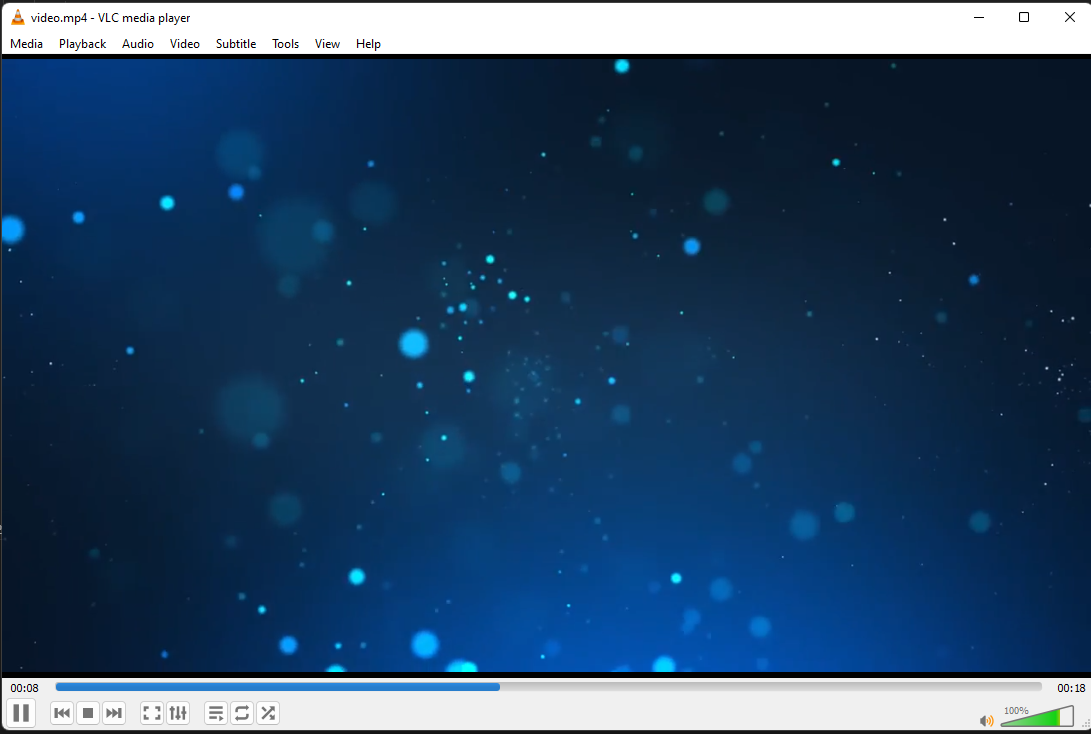
\includegraphics[width=0.95\textwidth]{images/image.png}
\caption{Input Video}
\end{figure}

Our watermark looks like this:

\begin{figure}[h!]
\centering
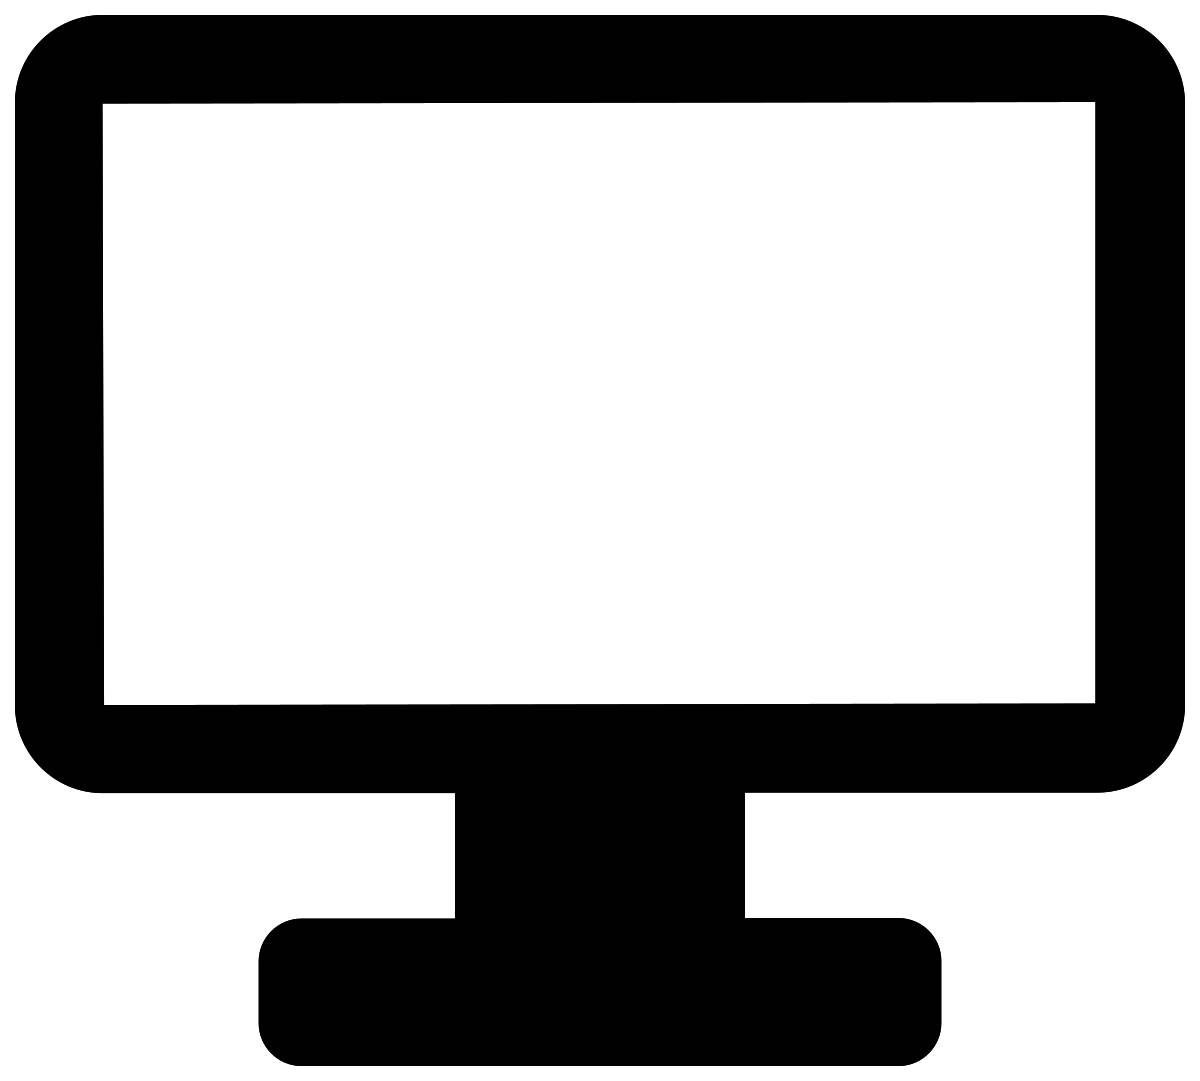
\includegraphics[width=0.8\textwidth]{images/watermarksample.png}
\caption{Input Watermark}
\end{figure}

The output video looks like this:

\begin{figure}[h!]
\centering
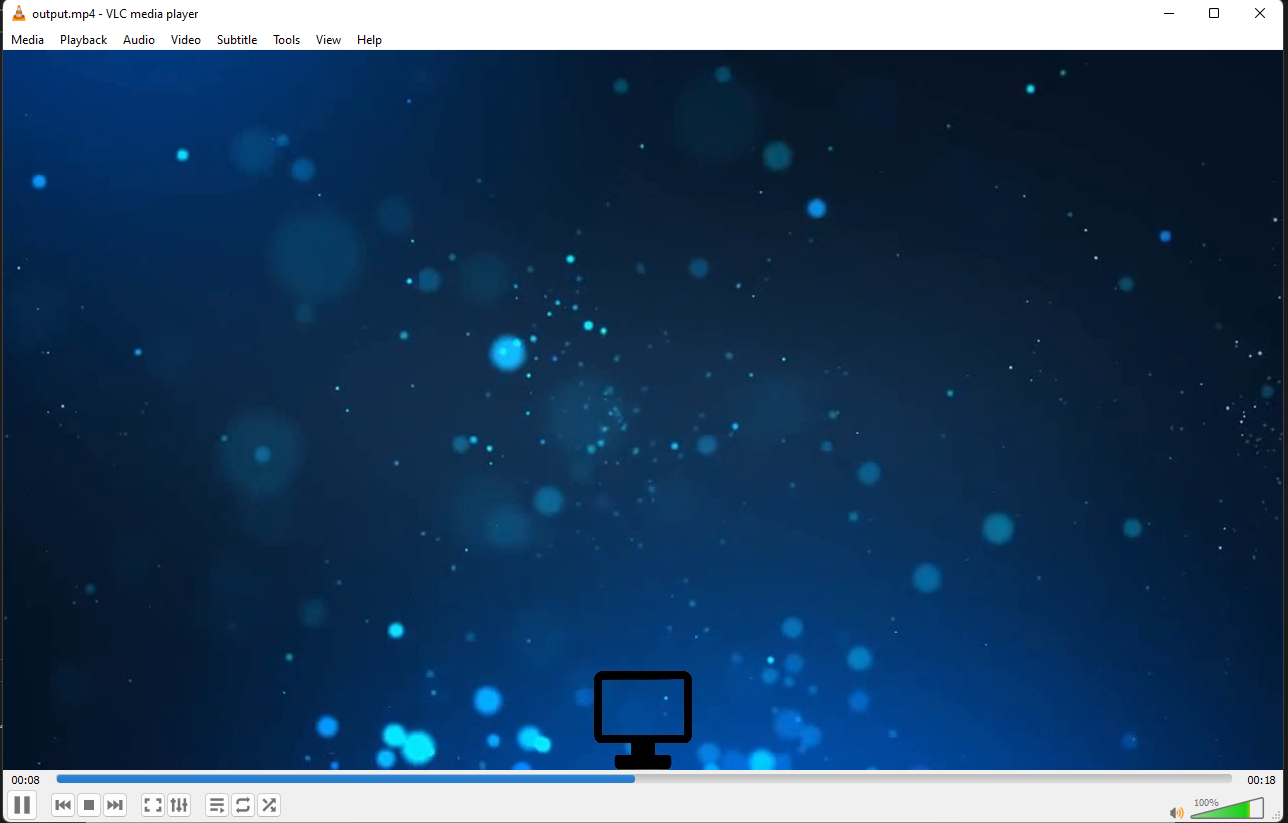
\includegraphics[width=0.95\textwidth]{images/image-2.png}
\caption{Output Video}
\end{figure}

\begin{markdown}
### Conclusion

In this notebook/paper, we have learned how to inject a watermark into a video
using Open-CV. Now i can successfully inject a watermark into a video.
The use case of this technique was to brand a video with a logo or a
watermark. This technique can be used to protect the video from being
copied or used without the permission of the owner.
\end{markdown}

\end{document}